\section{Pregunta N$^{\circ}$13\qquad Leon Alonzo Terrones Caccha}

\begin{frame}
    \begin{enumerate}\setcounter{enumi}{12}
        \item

              Obtenga el polinomio trigonométrico de mínimos
              cuadrados continuos $S_{3}\left(x\right)$ para
              \begin{math}
                  f\left(x\right)=
                  x^{2}\sin
                  \left(x^{2}\right)
              \end{math}
              en
              \begin{math}
                  \left[-\pi,\pi\right]
              \end{math}.
    \end{enumerate}

    \begin{solution}
        Deseamos obtener un polinomio trigonométrico de la forma:
        \[S_{3}\left(x\right)=\frac{a_{0}}{2}+a_{3}cos(3x)+\sum_{k=1}^{2}{a_kcos(kx)+b_ksen(kx)}\]
        donde:
        \[a_k=\frac{1}{\pi}\int_{-\pi}^{\pi}{f(x)cos(kx)}\]
        \[b_k=\frac{1}{\pi}\int_{-\pi}^{\pi}{f(x)sen(kx)}\]
    \end{solution}
\end{frame}
\begin{frame}{Results}
    \begin{figure}
        \centering
        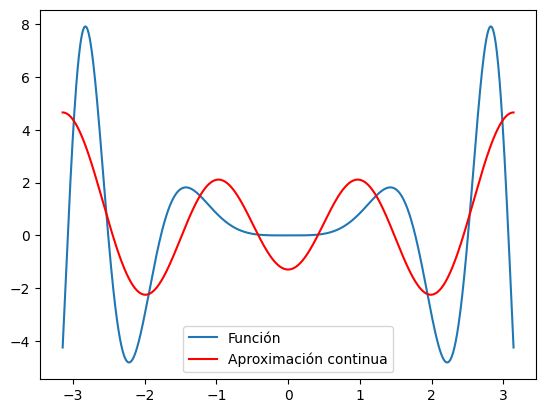
\includegraphics[width=8]{p13-Aprox-continua.png}
        \caption{Para $n=3$}
        \label{fig:enter-label}
    \end{figure}
\end{frame}
\begin{frame}{Results}
    \begin{figure}
        \centering
        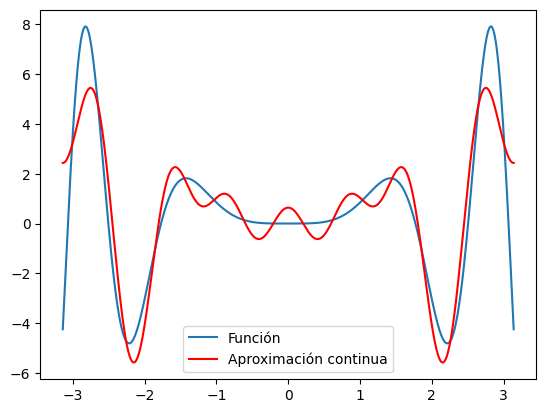
\includegraphics[width=8]{p13-A-continua.png}
        \caption{Para $n=7$}
        \label{fig:enter-label}
    \end{figure}
\end{frame}
\begin{frame}{Results}
    \begin{figure}
        \centering
        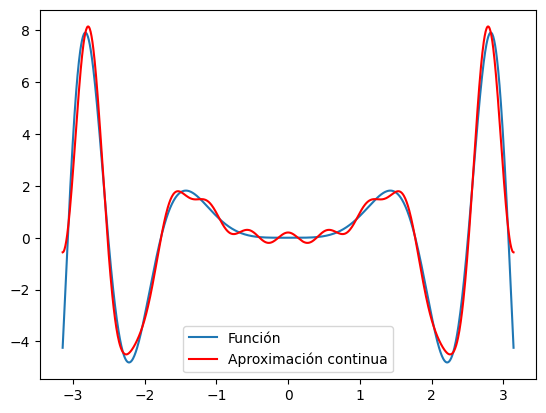
\includegraphics[width=8]{p13-A-cont3.png}
        \caption{Para $n=11$}
        \label{fig:enter-label}
    \end{figure}
\end{frame}